\documentclass{standalone}
\usepackage{tikz}
\begin{document}
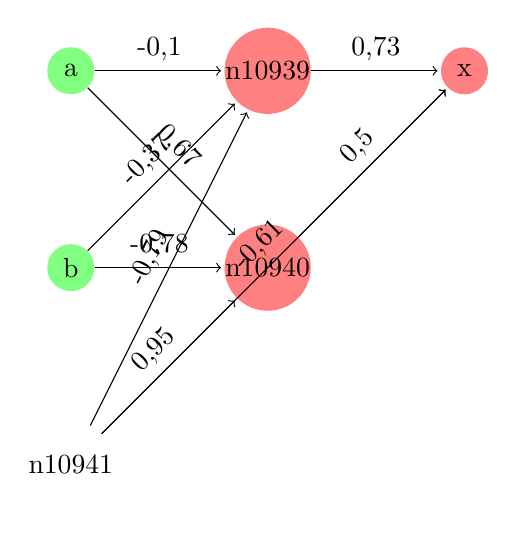
\begin{tikzpicture}[shorten >=1pt,->,draw=black!,node distance=2.5cm]
\tikzstyle{neuron}=[circle,fill=black!25,minimum size=17pt,inner sep=0pt]
\tikzstyle{constant}=[neuron, fill=white!50];
\tikzstyle{identity}=[neuron, fill=green!50];
\tikzstyle{sigmoid}=[neuron, fill=red!50];
\node [identity] (a) {a};
\node [identity,below of=a] (b) {b};
\node [constant,below of=b] (n10941) {n10941};
\node [sigmoid,right of=a] (n10939) {n10939};
\node [sigmoid,below of=n10939] (n10940) {n10940};
\node [sigmoid,right of=n10939] (x) {x};
\path[every node/.style={sloped,anchor=south,auto=false}]
(a) edge node {0,67} (n10940)
(a) edge node {-0,1} (n10939)
(n10941) edge node {-0,79} (n10939)
(n10941) edge node {0,95} (n10940)
(n10941) edge node {-0,61} (x)
(n10939) edge node {0,73} (x)
(n10940) edge node {0,5} (x)
(b) edge node {-0,78} (n10940)
(b) edge node {-0,37} (n10939)
;\end{tikzpicture}
\end{document}